\section{Operation Parameters}\label{sec:op-params}
%\lipsum[2-4]
As mentioned in the previous section:~\ref{sec:anchor-configurations} we determined the best anchor configurations for the given environment but the results were collected in an ideal scenario.
From work done by ~\citet{evaluwb} we can see that the major factor affecting the positional accuracy seems to be No Line Of Sight (NLOS) between the anchors and a tag at any given time.
                            %^TODO: Mention this in LR also?
Furthermore the work discusses the use of using an optimal triplet of anchors in order to improve accuracy this is an indication that a loss of a single anchor in the optimal configuration determined in the previous section should still yield reasonable results.
To confirm there operational parameters the following experiments were carried out.

\subsection*{Loss of Anchor}
In theory a minimum of three anchors are all that is needed for determining the two dimensional position, $(x,y)$, of the tag via trilateration.
Losing a single anchor would therefore allow for the $(x,y)$ position to be determined with a fair amount of accuracy with discrepancies showing up in the z position readings.
To test this data was recorded starting with all four anchors and then systematically one achor was turned of in each sample.
Figure:~\ref{fig:Loss_anchors} shows the plots obtained under this test.
It can be see that the $(x,y)$ position remains relatively unchanged in all with only a notable shift the z position with the loss of Anchor 1 and more noise introduced with the loss of Anchor 4.

\begin{figure}[h!]
    \centering
    \begin{subfigure}{0.45\textwidth}
            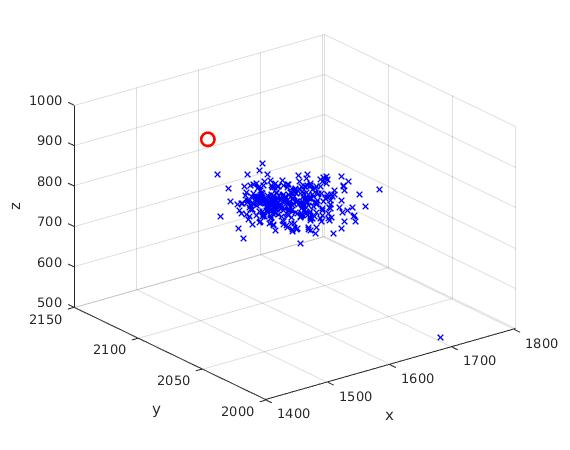
\includegraphics[width=\textwidth]{results/lossanchor1}
            \caption{Loss of Anchor 1}
    \end{subfigure}
    \begin{subfigure}{0.45\textwidth}
            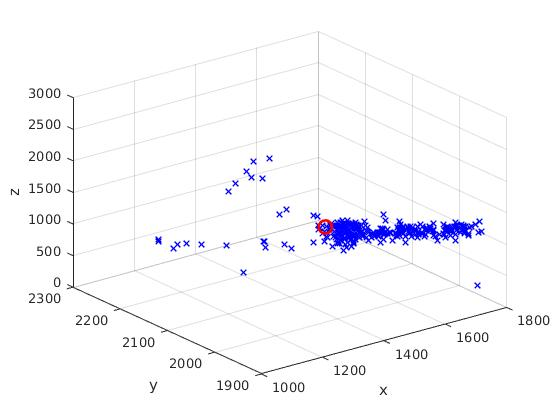
\includegraphics[width=\textwidth]{results/lossanchor2}
            \caption{Loss of Anchor 2}
    \end{subfigure}

    \begin{subfigure}{0.45\textwidth}
            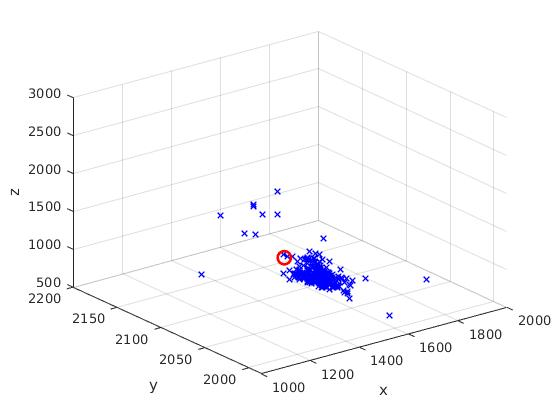
\includegraphics[width=\textwidth]{results/lossanchor3}
            \caption{Loss of Anchor 3}
    \end{subfigure}
    \begin{subfigure}{0.45\textwidth}
            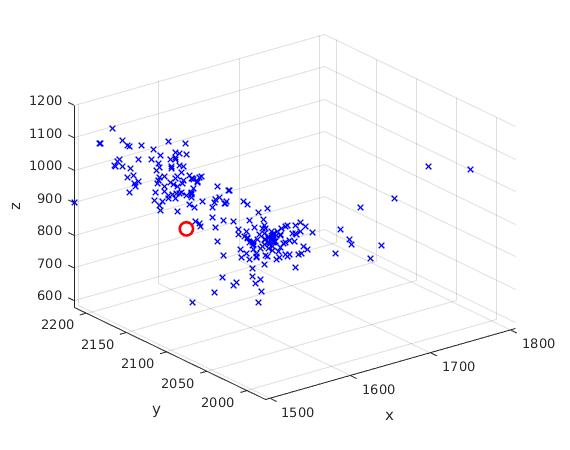
\includegraphics[width=\textwidth]{results/lossanchor4}
            \caption{Loss of Anchor 4}
    \end{subfigure}
    \caption{Results obtained when an Anchor was lost.}
    \label{fig:Loss_anchors}
\end{figure}
\newpage
\subsection*{No Line of Sight}
The positioning calculations are based on a Two way ranging and Time of flight Calculation scheme see Appendix:~\ref{app:app01}.
The major crux of the calculation is that the wave is always moving at the speed of light this means that introducing an obstacle between the any anchor and the tag that attenuates the signal would introduce discrepancies in the results obtained.
Figure:~\ref{fig:nlos} shows the setup used to test this scenario.
The system was allowed to record data with no obstacles then a person walked along the trajectory indicated by the dotted arrows in the Figure and came to a rest as seen.
It was ensured that the path taken by the person did not obstruct any of the anchors during motion.
This was carried out 3 times:
\begin{enumerate}
    \item Position 1: Provides NLOS between Anchor 2 and the tag.
    \item Position 2: Does not provide NLOS between any anchors and the tag.
    \item Position 3: Provides NLOS between Anchro 4 and the tag.
\end{enumerate}
Position 2 was done to confirm that no reflections or attenuation occur with a person just being in the proximity of the tag.
From Figure:~\ref{fig:persons} we can see that a person being introduced at position 1 and which obstructs line of sight between an anchor and the tag has adverse effects.
It is clear that the 2 distinct blobs seen in the plots for position 1 and 3 show that the tag's 'position' has changed although it is stationary.

\begin{figure}[h!]
    \centering
    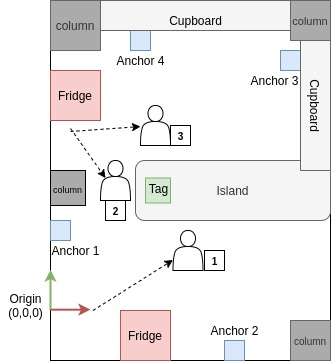
\includegraphics{mtd/loss_of_ppl}
    \caption{The test scenario for NLOS experiment}
    \label{fig:nlos}
\end{figure}

\begin{figure}[h!]
    \centering
    \begin{subfigure}{0.45\textwidth}
            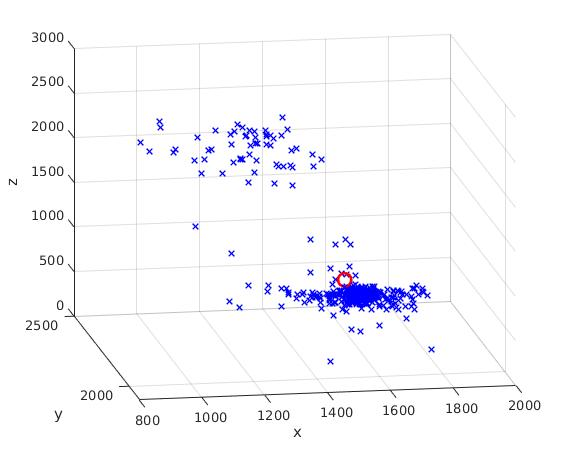
\includegraphics[width=\textwidth]{results/personatposition1}
            \caption{Person at Position 1}
    \end{subfigure}
    \begin{subfigure}{0.45\textwidth}
            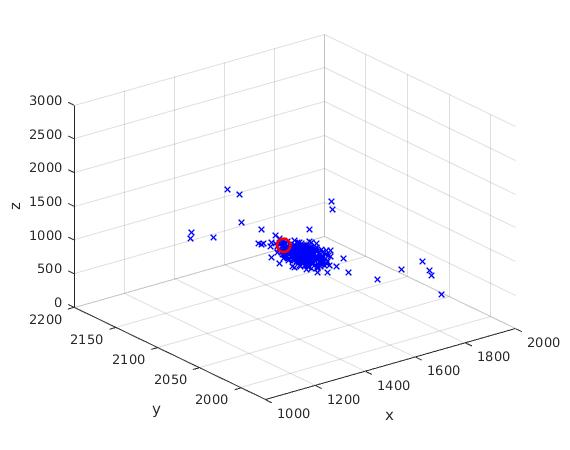
\includegraphics[width=\textwidth]{results/personatposition2}
            \caption{Person at Position 2}
    \end{subfigure}
    \begin{subfigure}{0.45\textwidth}
            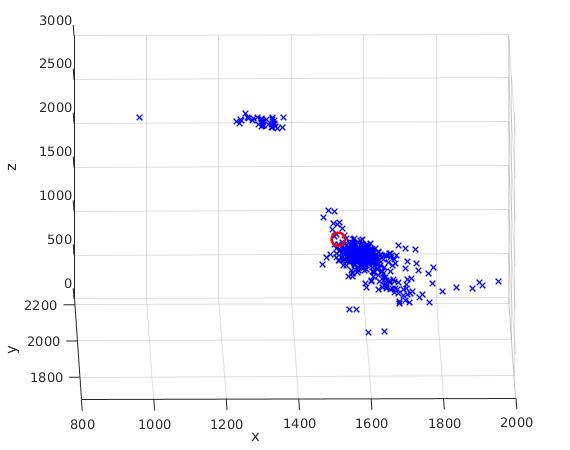
\includegraphics[width=\textwidth]{results/personatposition3}
            \caption{Person at Position 3}
    \end{subfigure}
    \caption{Results obtained when an Anchor was lost.}
    \label{fig:persons}
\end{figure}
As it stands, NLOS is the major factor affecting the operation of the system and the accuracy of the raw readings.
As such it is proposed that additional layers be added to procees this position data and try to improve the positional accuracy of the system and make it robust.

